\chapter{FileCatalog connected to a NoSQL database}
One of the main goals of this project was to test whether connecting the 
file catalog, more specifically its metadata part, to a NoSQL database would 
improve the feedback speed of the service thus making it more pleasant to use
or make it easier to implement and maintain. The new database had to satisfy the
following conditions in order to be connectable to DIRAC and deployable in
the computing centers.

\begin{itemize}
\item There has to be a free-ware version which could DIRAC use.
\item The database has to have a python interface or client so it would be easy
to incorporate it into DIRACs code.
\end{itemize}

The characteristics of the data itself add some restrictions. The database should be
optimized for search speed. When combined with the current metaquery implementation, we
get two different types of data retrieval. For directories 
the database has to be able to get all the metadata associated with a directory
identified by an ID. On contrary the files are fetched based on the terms in the metaquery so
all the querying techniques the metaquery could use have to be possible, including
range queries. 

\begin{figure}[h]
\centering
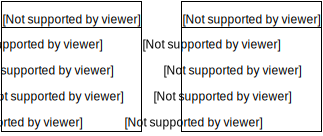
\includegraphics[scale=0.9]{img/dataTyp.pdf}
\caption{Theoretical data scheme in the metadata catalog}
\label{fig:theoDataScheme}
\end{figure}


\section{Apache Cassandra}
Apache Cassandra is a distributed database for managing large amounts of structured data 
across many commodity servers, while providing highly available service and no single point 
of failure \cite{cassandra}. Cassandra's data model is a
partitioned row store, rows are organized into tables. Each row
has an altering number of columns, which are essentially a
key-value pair, and is identified by a unique ID. Adding that Cassandra features
its own query language CQL (Cassandra Query Language) which resembles the standard SQL 
used by all relational databases, it looks like a perfect candidate for the metadata catalog.

\subsection{Developing a data model for Cassandra}

Although CQL makes it look like a relational database, the developer has to bare in mind, that
Cassandra is different. The first scheme used the altering number of columns and organized the 
data in tables, where each file or directory had its own row with metanames being the column
names and values being the column values (this model greatly resembles the theoretical data 
scheme in figure \ref{fig:theoDataScheme}) with secondary indexes over column values so that 
the query would be possible. Although the similarity with SQL would suggest otherwise, 
it turned out that this kind of indexing does not support range queries. 

After understanding more thoroughly how Cassandra works, another data model was introduced 
using most of Cassandras specific features. The only property Cassandra guaranties is that 
rows are not divided across multiple nodes in the cluster and column keys inside the row
are sorted. These two main characteristics lead to the functional data model. For  
directories row IDs are mapped on directory IDs and the model is similar to the previous one. 
Retrieving a row with given row ID is one of natively supported operations.
For files each metaname has its row, column names are meta values and column values are sets of 
file IDs of files having this metaname and value associated with them. 

\begin{table}[h]
\centering
\label{tab:fileMeta}
\begin{tabular}{|l|l|l|l|ll}
\hline
\multirow{2}{*}{Metaname A} & Value 1      & Value 2      & Value 3      & \multicolumn{1}{l|}{Value 4}      & \multicolumn{1}{l|}{Value 5}      \\ \cline{2-6}
                            & \{id,id,..\} & \{id,id,..\} & \{id,id,..\} & \multicolumn{1}{l|}{\{id,id,..\}} & \multicolumn{1}{l|}{\{id,id,..\}} \\ \hline
\multirow{2}{*}{Metaname B} & Value 1      & Value 2      & Value 3      &                                   &                                   \\ \cline{2-4}
                            & \{id,id,..\} & \{id,id,..\} & \{id,id,..\} &                                   &                                   \\ \cline{1-4}
\end{tabular}
\caption{File metadata}
\end{table}

The rows are grouped
in tables by value type, because the algorithm used to sort the
column names has to be unified per table. There also is an index over fileID sets, 
so that retrieving all metadata for one specific file is possible, but the scheme is 
not optimized for this operation.



\begin{lstlisting}[language=sql, caption=Data structure described by CQL]
CREATE TABLE file_int (
    metaname text,
    value int,
    fileid set<int>,
    PRIMARY KEY (metaname, value)
);
\end{lstlisting}

In CQL this structure looks like a table with three columns and a compound primary key which
brings the main disadvantage of this approach: meta names can be queried only one at a time and
the result has to be then composed in the code of the application.

\begin{lstlisting}[language=sql, caption=Example query]
SELECT fileid 
	FROM file_int 
	WHERE metaname='metaInt1' AND value>3;
\end{lstlisting}

\section{MongoDB}

\section{Elasticsearch}

